In this chapter, we provide information regarding the experimental setup and performance evaluation. To be more precise, this chapter explains which data set we use, how the data is partitioned, which models are used in the experiments, the software and hardware specifications of the experimental environment, as well as description of experiments we perform.

\section{Data Set}\label{eval:data_set}

The data set used for the experiments is the MNIST \cite{lecun2010mnist} data set. The MNIST data set includes 70,000 images of handwritten digits from 0 to 9, where each image is 28 by 28 pixels. Some samples are illustrated in \autoref{fig:mnist}.

\begin{figure}[!htp]
    \centering
    \centering
    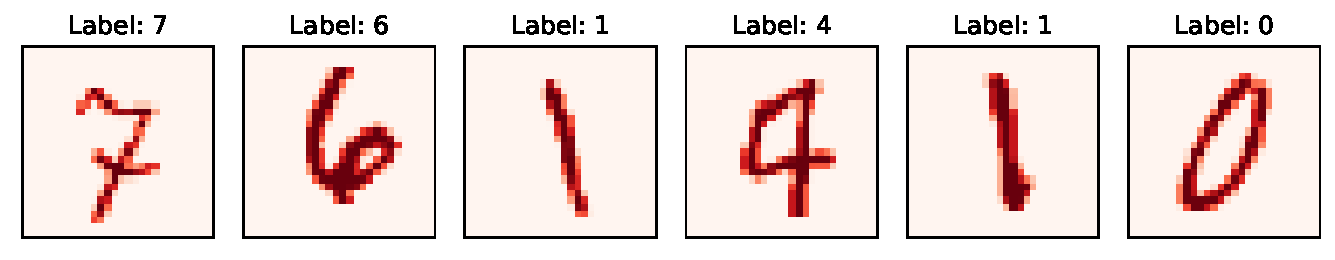
\includegraphics[width=1\textwidth]{graphics/mnist.pdf}
    \caption{MNIST Example Samples}
    \label{fig:mnist}
\end{figure}

The MINST data set is not only a well-known data set but also widely used by the majority of the reviewed works, as seen in \autoref{tab:data_distribution}. Therefore, to be able to compare our experiment results with the original works, we use the same data set.

\section{Client Sampling}\label{eval:client_sampling}

The client sampling, that is, the process of dividing the samples among the clients, depends on how data is partitioned across federated learning clients. Data may be partitioned horizontally or vertically in federated learning systems. In the following subsections, we explain how we sample the data for each of the data partitions.

\subsection{Horizontal}

In horizontally partitioned data, as explained in \Cref{background:archfl}, different clients have different samples that share the same feature space. Additionally, in a distributed system, it is expected that the clients are heterogeneous in terms of their computational characteristics and data. Therefore, it is safe to assume that the data distribution in a distributed setting is \textit{non-iid}.

To simulate a \textit{non-iid} distribution, both in terms of number of samples and number of classes at each client, we use the Dirichlet distribution \cite{tim, 10.48550/arxiv.2006.07242}. The Dirichlet distribution, $Dir(\alpha)$, is a probability distribution characterized by its parameter $\alpha$, which controls the degree of \textit{non-iid}-ness of the distribution. The higher the $\alpha$, the more identically distributed the data will be. The lower the $\alpha$, the more likely it is for each client to only hold samples of a single class.

For our experiments, we set $\alpha = 0.1$ in the Dirichlet distribution as it yields a realistic \textit{non-iid} distribution \cite{10.48550/arxiv.2006.07242}, where some clients hold many samples of a few classes, while other clients have few samples of many classes. Moreover, the clients have, on average, 2500 samples each. Some clients have more samples, some have less, simulating a \textit{non-iid} distribution.

In order to perform the horizontal client sampling, we used a publicly available tool \cite{tsingz0} that supports sampling from the MNIST data set directly using the Dirichlet distribution. We did so for 5, 10, 25 and 50 clients. \autoref{fig:horizontal_dist} illustrates the sample distribution for 10 clients. From \autoref{fig:horizontal_dist}, it is possible to see how \textit{non-iid} the distribution is, both in terms of number of data samples and class distribution. For example, client 7 has many samples from classes 2 and 4, while having none of the remaining classes. At the same time, client 10 has a few samples from classes 0, 1, 2, and 9 and many from class 7.

\begin{figure}[!ht]
    \centering
    \centering
    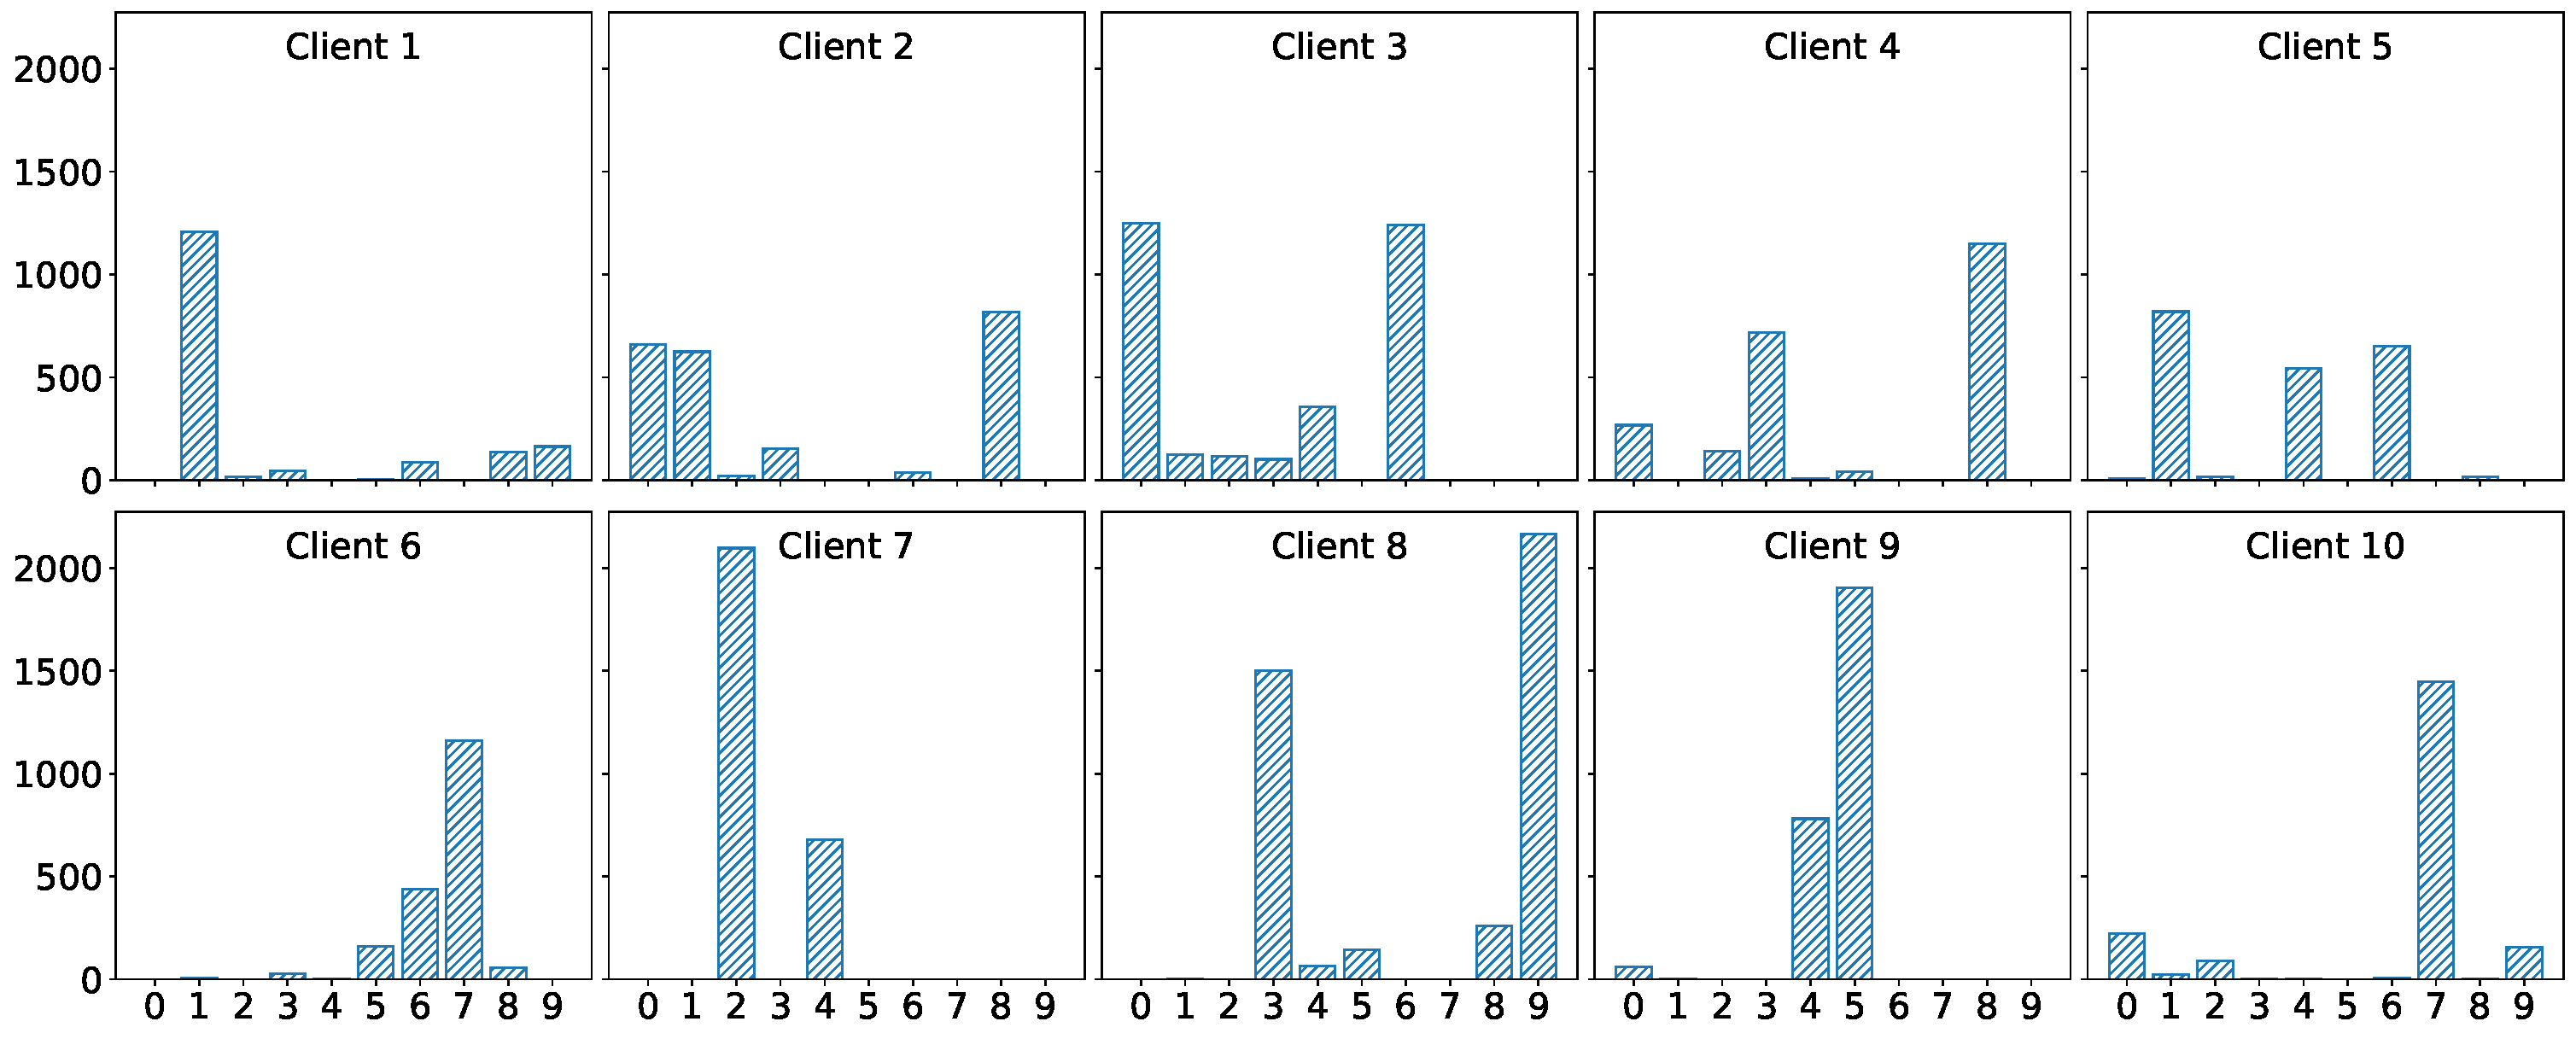
\includegraphics[width=1\textwidth]{graphics/10_dist.pdf}
    \caption{Horizontal Data Distribution For 10 Clients}
    \label{fig:horizontal_dist}
\end{figure}

\subsection{Vertical}\label{subsection:verticalpartitioning}

Vertically partitioned data is significantly different from horizontally partition data, in the sense that the clients share intersecting sample spaces, but different feature spaces. Therefore, it is not possible to simply divide the samples among the clients.

\begin{figure}[!ht]
    \centering
    \centering
    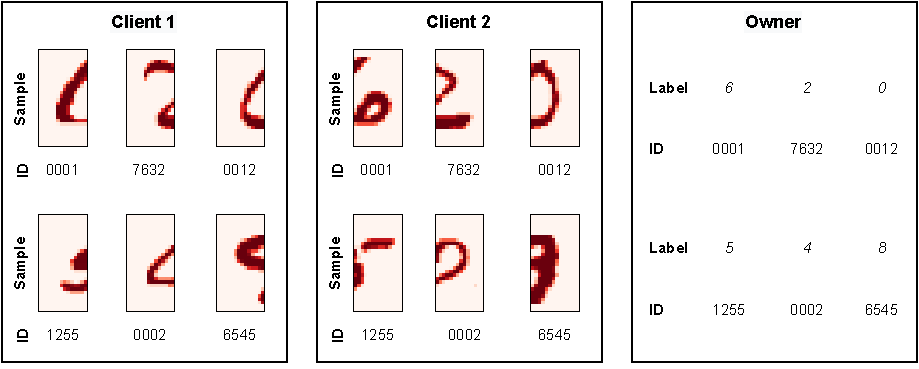
\includegraphics[width=1\textwidth]{graphics/vertical_partitioning.pdf}
    \caption{Vertical Data Distribution for 2 Clients}
    \label{fig:vertical_dist}
\end{figure}

For the vertical data partition, we use the work reported in \cite{10.48550/arxiv.2104.00489}. Firstly, we choose how many samples to assign to each client. We chose 20,000 samples in order to match the original work \cite{10.48550/arxiv.2104.00489} we will be comparing to. Then, the samples are randomly chosen from the original data set. Subsequently, each sample is assigned a unique identifier (ID) that will be used as label when giving the data samples to each client. Only the servers have access to the ground truth labels. After assigning the IDs, the feature space $F$ will be divided into $C$ parts $F_c$, where $C$ is the number of clients. Finally, the features $F_c$, with $c \in C$ will be assigned to each of the clients.

For vertical data partitioning, we divide the data set as in \cite{10.48550/arxiv.2104.00489} to use it with a Split-CNN \cite{10.1145/3297858.3304038} model, which will be introduced in the next section. To use this model, the model owner is expected to have the labels, while the clients are expected to have some features of each sample. For the MNIST data set, we can think of the features as vertical fragments of the image. To divide a 28 by 28 image sample between 2 clients, for example, we split the image into two 14 by 28 segments, as depicted in \autoref{fig:vertical_dist}.

\section{Machine Learning Models}\label{eval:ml_models}

The models used on this work are simple models found in related work. The goal of this work is not to provide the most efficient or accurate FL model. Therefore, we do not dive into the details of the models. The models used for horizontal and vertical training are succinctly explained below.

\subsection{Horizontal Model}

For the horizontal FL, we use a simple Convolutional Neural Network (CNN) \cite{cnn} with three levels of convolution intercalated with max pooling to reduce overfitting. These layers are followed by a flattening layer and two dense layers that culminate in the output. The architecture is depicted in \autoref{fig:model_cnn} and more details about its parameters can be found in \autoref{tab:cnn}. To train this model, both servers and clients have the same model. Then, the clients train the the model with their own data set. Subsequently, the clients send the weights to the servers by submitting their local model update to the blockchain via the smart contract. Finally, the servers aggregate the weights and publish the global model weights through the smart contract.

\begin{figure}[!hb]
    \centering
    \centering
    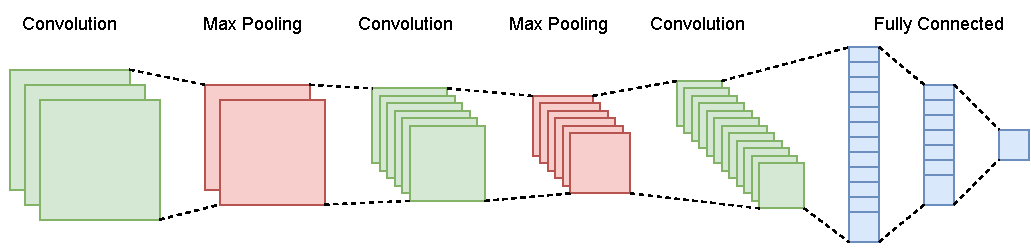
\includegraphics[width=1\textwidth]{graphics/model-cnn.pdf}
    \caption{CNN Model Architecture}
    \label{fig:model_cnn}
\end{figure}

\begin{table}[!h]
    \begin{tabular}{c|c}
        \hline \hline
        Layer Type       & Output Shape \\ \hline \hline
        Convolutional 2D & (26, 26, 32) \\ \hline
        Max Pooling 2D   & (13, 13, 32) \\ \hline
        Convolutional 2D & (11, 11, 64) \\ \hline
        Max Pooling 2D   & (5, 5, 64)   \\ \hline
        Convolutional 2D & (3, 3, 64)   \\ \hline
        Flatten          & (576)        \\ \hline
        Dense            & (64)         \\ \hline
        Dense            & (10)         \\ \hline
    \end{tabular}
    \caption{CNN Model Parameters of the Horizontal FL}
    \label{tab:cnn}
\end{table}

\subsection{Vertical Model}

For the vertical FL, we use a dual-headed, or four-headed, Split-CNN \cite{10.1145/3297858.3304038, 10.48550/arxiv.2104.00489}, depending on whether we have two or four clients. The model at the clients is the head model, while the model at the servers is the tail model. To train this model, each client gives its input data to the models and collects the output of the last layer. Then, this intermediate output is sent to the servers, which are then given to the tail model. The servers calculate the gradients, which are then backpropagated to the clients. For more details, please consult the original works where the workings of this model are given in more detail. The architecture is depicted in \autoref{fig:model_splitcnn} and more details about its parameters can be found in \autoref{tab:splitnn}.

\begin{figure}[!ht]
    \centering
    \centering
    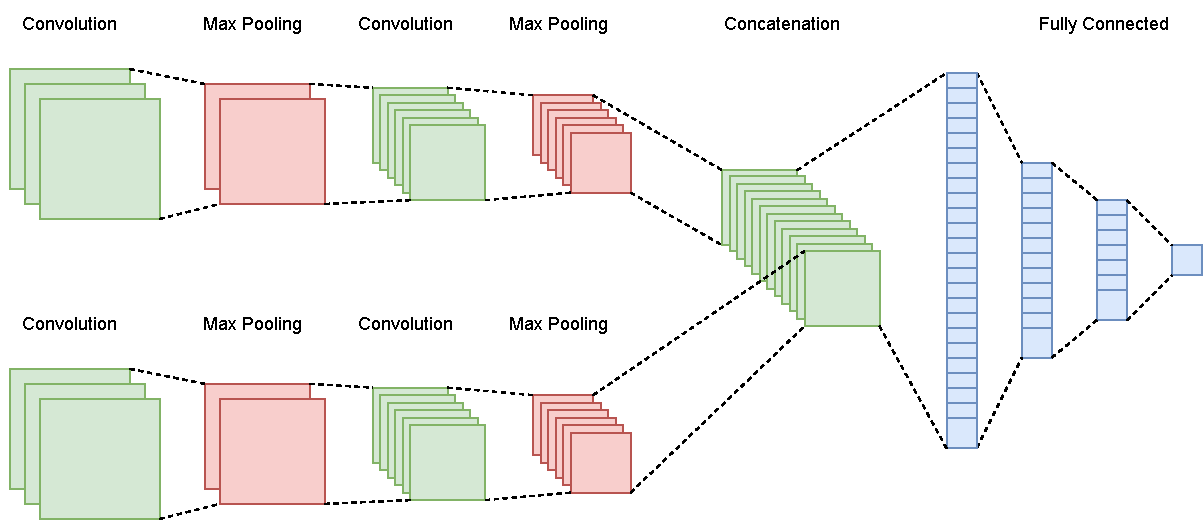
\includegraphics[width=1\textwidth]{graphics/model-splitcnn.pdf}
    \caption{Split-CNN Model Architecture}
    \label{fig:model_splitcnn}
\end{figure}

\begin{table}[!h]
    \begin{subtable}[h]{0.49\textwidth}
        \centering
        \begin{tabular}{c|c}
            \hline \hline
            Layer Type       & Output Shape \\ \hline \hline
            Convolutional 2D & (26, 12, 32) \\ \hline
            Max Pooling 2D   & (13, 6, 32) \\ \hline
            Convolutional 2D & (11, 11, 64) \\ \hline
            Max Pooling 2D   & (5, 2, 64)   \\ \hline
        \end{tabular}
        \caption{Head}
    \end{subtable}
    \hfill
    \begin{subtable}[h]{0.49\textwidth}
        \centering
        \begin{tabular}{c|c}
            \hline\hline
            Layer Type     & Output Shape \\ \hline\hline
            2 Input Layers & (5, 2, 64)   \\ \hline
            Concatenation  & (5, 2, 128)  \\ \hline
            Flatten        & (1280)       \\ \hline
            Dense          & (512)        \\ \hline
            Dense          & (256)        \\ \hline
            Dense          & (10)         \\ \hline
        \end{tabular}
        \caption{Tail}
     \end{subtable}
     \caption{Split-CNN Dual-Headed Model}
     \label{tab:splitnn}
\end{table}

\section{Hardware and Software Specifications}

The experiments were executed in a remote machine, whose hardware and software specifications can be found in \autoref{tab:temps}. Due to resource limitations, it was not possible to have a machine with GPU. Furthermore, if we consider that FL systems are being run in IoT clients, it is unlikely that such resource-constrained devices would have a GPU available. In addition, the MNIST data set and the models we used are relatively simple, which means that they can be easily trained using CPUs. Nonetheless, it is worth mentioning that the training process would likely be faster in machines with GPUs.

\begin{table}[!h]
    \begin{subtable}[h]{0.59\textwidth}
        \centering
        \begin{tabular}{l|l} \hline \hline
            Hardware & Model                                    \\ \hline \hline
            CPU      & AMD Ryzen 5 3600 6-Core 4.2 GHz          \\ \hline
            RAM      & 64 GB                                    \\ \hline
            Disk     & 500 GB NVMe                              \\ \hline
        \end{tabular}
        \caption{Hardware}
        \label{evaluation:hardware}
    \end{subtable}
    \hfill
    \begin{subtable}[h]{0.39\textwidth}
        \centering
        \begin{tabular}{l|l} \hline \hline
            Software            & Version               \\ \hline \hline
            Docker              & 20.10.15              \\ \hline
            Docker Compose      & 2.5.0                 \\ \hline
            Python              & 3.8.13               \\ \hline
            Node.js             & 16.15.0               \\ \hline
            Truffle             & 5.5.13               \\ \hline
            Ganache             & 7.1.0               \\ \hline
            Solidity            & 0.5.16               \\ \hline
        \end{tabular}
        \caption{Software}
        \label{evaluation:software}
     \end{subtable}
     \caption{Hardware and Software Specifications of Experiments}
     \label{tab:temps}
\end{table}

\section{Performance Evaluation Metrics}\label{eval:metrics}

We select the following metrics for our performance evaluation: execution time, transaction costs, transaction latency, model accuracy and convergence, communication costs, and computation costs.

\subsection{Execution Time}

To compare execution time, we define two metrics: the \textit{End-to-end (E2E) Execution Time} and the \textit{Mean Round Execution Time}. The former is defined by the time it takes for an experiment to be executed from start to the end. The latter is defined by the mean time it takes to complete an experiment round, which can be calculated by dividing the E2E Execution Time by the number of rounds of the experiment.

\subsection{Transaction Costs and Transaction Latency}

To compare the blockchain costs, namely the impact of waiting for transactions, we define two metrics: the \textit{Transaction Latency} and the \textit{Transaction Cost}. The former is defined as the mean time it takes between submitting a transaction and it being accepted by the network. The latter is defined by the mean computation effort to execute a transaction, which, in the case of Ethereum, is measured in \textit{Gas}.

Both the transaction latency and transaction cost values are retrieved directly from the Blockchain. Ethereum provides information on how much time transactions take to be accepted, as well as how much each transaction costs. Then, we only calculate the mean.

\subsection{Model Accuracy}

To compare the model accuracy, we use a global \textit{Accuracy} metric for the FL model, where the model owner, that is, the one that initiates the process, has some data set with which it can test the model. The logs produced by the model owner contain the accuracy and are used to extract the accuracy of each round.

\subsection{Communication and Computation Costs}

To compare the communication costs, we define the \textit{Network Traffic Per Round} metric, which is defined by how much network traffic flows to and from each process. It is collected for the client, server, and blockchain processes individually. By knowing the network traffic required for each process, we can draw conclusions regarding how the network traffic impacts different types of devices. For example, if there is a high volume of traffic per round at the client process, and the clients are resource-constrained IoT devices with low network bandwidth, then it is expected that each round takes longer since less traffic can go through the device at a single point in time.

To compare the computation costs, we collect the \textit{RAM Usage} and \textit{CPU Usage}.

The communication and computation costs metrics are collected at the client, server, and blockchain processes in order to be able to differentiate the effects of the different algorithms on the different parts of the system. However, it is important to note that, in practical settings, the server process and the blockchain process run on the same device.

To collect these metrics, we use \texttt{docker stats}, which is a command provided by Docker, the platform used for BlockLearning's Testbed. The statistics command provides a live stream of the container's resource consumption, namely the CPU percentage, the RAM memory usage, and the network traffic in and out.

\section{Experiment Groups}\label{meth:experiments}

The conducted experiments can be divided into three groups, of which two analyze how using different types of algorithms impact the system's performance in terms of model accuracy, convergence, communication, and computation costs. These two groups relate to impact analysis of:

\begin{enumerate}
    \item \textit{Consensus Algorithms}: PoA, PoW, and QBFT. Consensus algorithms are a component of the blockchain and they are expected to impact Horizontal Federated Learning and Vertical Federated Learning equally.
    
    \item \textit{Horizontal Federated Learning}
    
    \begin{enumerate}
        \item \textit{Participant Selection Mechanisms}: random selection versus first-come first-served.
        
        \item \textit{Scoring Algorithms}: BlockFlow, Multi-KRUM, Marginal Gain, as well as without any scoring algorithm. For each scoring algoritm, we also analyse the impact of:
        
        \begin{enumerate}
            \item \textit{Number of Clients}: 5, 10, 25, 50, selected based on the current literature and available resources we have at our disposal to execute the experiments.
            
            \item \textit{Privacy Degree}: 1 and 5, as well as without any privacy mechanism.
        \end{enumerate}
    \end{enumerate}
\end{enumerate}

In the third and last experiment group, we investigate if it is possible to implement and run a Blockchain-based Federated Learning with vertically partitioned data. To do so, we analyze how to extend the BlockLearning framework in order to support the Split-CNN model. Then, we implement the required extensions to the framework. Finally, we execute the experiments and compare the results with the original work where the Split-CNN model was used with the MNIST dataset in order to validate our experiment.

As explained in \Cref{background:archfl}, Vertical Federated Learning systems have an additional step, in which the Private Set Intersection (PSI) of the client's data sets is calculated. In this work, we assume that the PSI is calculated beforehand and that it is already known to all devices. The PSI calculation can be done in different ways and it is its own area of research of Computer Science. The related works we analyzed either did not provide information on how this was calculated, or also assumed that is has been calculated beforehand. In future works, it would be interesting to integrate a PSI mechanism into the framework.

All experiments were performed for 50 rounds so that we can compare the model accuracy results to other papers. This way, we can validate if our experiments are within the expected values. Secondly, all experiments were performed with 10 servers that run both the server process and the blockchain process. Thirdly, all experiments, except for those where the number of clients are compared, are run with 25 clients.
